
\newcommand*\circled[1]{
  \tikz[baseline=(C.base)]\node[draw,circle,inner sep=1.2pt,line width=0.2mm,](C) {#1};}
%sigue haciendo colision?...
\newcommand*\Myitem{
  \stepcounter{enumi}\item[\circled{\theenumi}]}
\centering
\flushleft{\section{Raíces en 1D}}
 \raggedright
\underline{Def:}
La función \(f(x)\) tiene una raíz en \(x = r\) si \(f(r) = 0\).\\
\underline{Th:} Sea \(f\) una función continua en \([a,b]\), satisfaciendo \(f(a) \cdot f(b) < 0\). Entonces \(f\) tiene una raíz entre \(a\) y \(b\); es decir, existe un número \(r\) que satisface \(a < r < b\) y \(f(r) = 0\).\\
\vspace{0.5cm}
\underline{Ej:} \(f(x) = x^{3} + x - 1\)\\
\begin{center}
\begin{tikzpicture}
    		%ejes
    		\node[anchor=east] at (0.0,0.0) (origenreal) {}; %origen
    		\node at (-0.2,0.1) (origen) {};	
  		%%%% EJES!!!
  		\draw [->] (-3,0) -> (5,0);
  		\draw [->] (0,-3) -> (0,3);
  		%%%PARABOLA
  		\node[anchor=east] at (0,-1.5) (iii) {f(x)};
  		\node[anchor=east] at (5,2) (ddd) {};
  		%%%DIBUJO PARABOLA
  		\draw (iii) edge[-,out=0,in=240] (ddd);
  		%\draw (invo) edge[->,out=90,in=270] (invy);
  		\node[anchor=east] at (5.5,0) (x) {x};
  		\node[anchor=north] at (0,3.5) (y) {y};
  		\node[anchor=east] at (5,-0.2) (x) {b};
  		\node[anchor=east] at (0,-0.2) (x) {a};
  		\node[anchor=east] at (3,-0.2) (x) {c};
  		\node at (0.0, 2) (oy) {};
\end{tikzpicture}
\end{center}
\hspace{8cm}$\Uparrow$\\
\hspace{7cm}\(f(r) = 0\),\\
\hspace{6cm}¿Cómo obtengo r?\\
\begin{center}
\hspace{1cm} Digamos \(a = 0\), \(f(a) = -1\) y \(f\) es continua.\\
\vspace{0.5cm}\hspace{1cm} \(b = 1\), \(f(b) = 1 \)\\
\vspace{0.5cm}
$\Rightarrow$ \(f(a) \cdot f(b) = (-1) \cdot 1 = -1 < 0\)\\
\vspace{0.5cm}
$\therefore$ Existe una raíz entre \(a < r < b\).\\
\end{center}
%Fin pag1
\newpage
\subsection{Método de la Bisección}
\vspace{0.5cm}
\raggedright

¿Como puede localizar un nombre en un directorio telefonico desconocido? Para 
buscar "Smith", puede comenzar por abrir el directorio al azar, por ejemplo 
abrirlo en la letra Q. Acontinuacion se puede seguir buscando en más hojas y terminar en la letra 
U. Ahora se tiene confinado el apellido "smith" entre las letras Q y U, por lo que debe centrar su 
búsqueda, mediante limites más pequeños que finalmente llevaran al apellido "Smith". El metodo de 
la biseccion representa este razonamiento, realizado de la manera mas eficiente posible.\\
\vspace{0.2cm}
Dado un intervalo inicial \([a, b]\) y \(f(a) \cdot f(b) < 0\), el algoritmo para el metodo de la biseccion es:\\

\begin{algorithm}
\begin{algorithmic}[1]
  \WHILE{\((b-a)/2 > TOL\)}
    \STATE $c = (a + b)/2$
  \IF{\(f(c) = 0\)}
    \STATE stop, end
  \ENDIF
  \IF{\(f(a) \cdot f(c) < 0\)}
    \STATE $b = c$
  \ELSE
    \STATE $a = c$
  \ENDIF
  \ENDWHILE
\end{algorithmic}
\end{algorithm}

\vspace{0.5cm}
\begin{itemize}
\item El intervalo final \([a, b]\) contiene una raíz. \\   
\item La aproximación a la raíz es \(r \approx \frac{(a + b)}{2}\)\\
\end{itemize}
\vspace{0.5cm}
¡Ver iPython notebook!\\
\vspace{0.5cm}
\hspace{1cm} \textbf{¿Qué tan exacto y qué tan rápido es el metodo de la biseccion?}\\
\vspace{0.3cm}
\underline{Bisección:} 
\begin{itemize} 
	\item Largo intervalo inicial \((b-a)\)\\
	\item Largo intervalo 1era iteración \(\frac{(b-a)}{2}\)\\
	\item \hspace{2cm}\( \vdots \) \\
	\item Largo intervalo tras $n$-ésima iteración $\frac{(b-a)}{2^n}$
	\vspace{0.5cm}
\end{itemize}
Luego de \(n\) pasos tenemos que el error de la solucion sera:\\
\vspace{0.2cm}
\hspace{0.5cm} Error de la solución: $ \displaystyle |x_c - r| < \frac{(b-a)}{2^{n+1}}$\\
\vspace{0.5cm}

%fin pagina 2
\newpage
\hspace{1.5cm} donde \( \displaystyle x_c = \frac{a_n + b_n}{2}\)\\
\vspace{0.5cm}
\hspace{1cm} y requiere \(n+2\) evaluaciones de \(f\).\\
\vspace{0.5cm}

Una buena forma para evaluar la eficiencia del metodo, es preguntarse cuanta precision puede obtenerse por cada evaluacion de la funcion. En cada evaluacion de la funcion se reduce la incertidumbre en la raiz por un factor de dos.\\
\vspace{0.5cm}

\underline{Def:} Una solución es correcta en \(p\) decimales si el error es menor que \(0.5 \cdot 10^{-p}\).\\
\vspace{0.5cm}
\underline{Ej 1.2:} Use el método de la Bisección para encontrar una raíz de \(f(x) = \cos{x} - x\) en el intervalo \([0, 1]\) correcta en 6 decimales.
\begin{center}
$\Rightarrow |x_c - r| < \frac{1-0}{2^{n+1}} < 0.5 \cdot 10^{-6}$\\
\vspace{0.5cm}
$\Rightarrow n > \frac{6}{\log_{10}2} \approx 19.9$\\
\vspace{0.5cm}
\hspace{1cm} $\therefore n = 20.$
\end{center}
¡Ver iPython notebook!
\subsection{Iteración de Punto Fijo}
Aplique la funcion ``\(\cos\)'' en una caculadora (¡asegurese de que este en radianes!) repetidas veces a un numero de inicio arbitrario, es decir aplicar la funcion cos al numero de inicio, luego al resultado y luego al nuevo resultado y asi sucesivamente, despues de cierto numero de iteraciones notara que el numero no cambia, es decir converge a un numero en especifico. En esta seccion se dara  una explicacion a este fenomeno, el cual es un ejemplo de iteracion de punto fijo.     

\raggedright
\subsection*{Punto fijo de una Función}
\underline{Def:} El número real ``r'' es un punto fijo de la función \(g(x)\) si \(g(r) = r\).\\
%\vspace{0.5cm}
\subsection*{Iteración de punto fijo}
\(x_0\) = ``Initial guess"\\
\(x_{i+1} = g(x_i),\,\, i = 0, 1, 2, ..., \infty\)\\
%\vspace{0.2cm}
Por lo tanto:\\
\begin{equation*}
	\begin{aligned}
		i = 0: x_1 &= g(x_0)\\ 
		i = 1:\,\, x_2 &= g(x_1) \\
		i = 2:\,\, x_3 &= g(x_2) \\
 		\vdots \\ 
 		i = n:\,\, x_{n+1} &= g(x_n) 
	\end{aligned}
\end{equation*}

%Fin página 3
\newpage
La secuencia $x_i$ puede converger o no a medida que el numero de pasos tiende a infinito. Sin embargo si $g$ es continua y las $x_i$ convergen a un numero $r$, entonces $r$ es un punto fijo.\\
\vspace{0.5cm}
\fbox{\parbox[c]{15cm} {\emph{\underline{Th:} Sea \(f\) una función continua en un vecindario de \(x_0\), y asume que $\displaystyle\lim_{n \to \infty} x_n = x_0$. Entonces,}
$$  \displaystyle\lim_{n \to \infty} f(x_n) = f(\lim_{n \to \infty} x_n) = f(x_0)$$}}\\
\vspace{0.2cm}
$\Rightarrow g(r) = g(\displaystyle\lim_{i \to \infty} x_i) = \lim_{i \to \infty} g(x_i) = \lim_{i = \infty} x_{i+1} = r$\\
\vspace{0.2cm}
Por lo tanto para nuestro ejemplo inicial de la funcion coseno, tenemos que la iteracion de punto fijo quedara definida como:\\
\vspace{0.2cm}
$\therefore x_{i+1} = \cos{(x_i)} \Rightarrow g(x) = \cos{(x)}$ y $f(x) = x-\cos{(x)} $\\

\centering
\subsection*{Ejemplo para \(x^3 + x - 1 = 0\)}
\vspace{1.5cm}
\begin{enumerate}
\Myitem
\hspace{6cm}\(x = 1 - x^3 = g_1(x)\) \\
\vspace{0.5cm}
\Myitem
\hspace{6cm}\(x = \sqrt[3]{1-x} = g_2(x)\)\\
\Myitem
\begin{equation*}
\begin{aligned}
x^3 + x - 1 &= 0 \hspace{1cm}/ +1 \\
x^3 + x &= 1 \hspace{1cm}/ +2x^3 \\
3x^3 + x &= 1 + 2x^3 \\
x(3x^2 + 1) &= 1 + 2x^3 \\
x &= \frac{1 + 2x^3}{1 + 3x^2} = g_3(x)
\end{aligned}
\end{equation*}
\end{enumerate}
%Fin página 4 
\newpage
\raggedright
\subsection{Geometría de la iteración de Punto Fijo (cobweb diagram)}
\centering
\begin{tikzpicture}
    		%ejes
    		\node[anchor=east] at (0.0,0.0) (origenreal) {}; %origen
    		\node at (-0.2,0.1) (origen) {};
  		%%%% EJES!!!
  		\draw [] (-0.5,0) -> (8,0);
  		\draw [] (0,-0.5) -> (0,6);
  		%\draw [] (0,0) -> (6,6);
  		\draw [] (0, 5.5) -> (7.2, 0);
  		\draw [] (2.5,0) -> (2.5, 3.6);
  		\draw [] (2.5, 3.6) -> (4.8, 3.6);
  		\draw [] (4.8, 3.6) -> (4.8, 1.8);
  		\draw [] (4.8, 1.8) -> (2.35, 1.8);
  		\draw [] (2.35, 1.8) -> (2.35,3.7);
  		\draw [] (2.35,3.7) -> (5,3.7);
  		\draw [] (5,3.7) -> (5,1.6);
  		\draw [] (5,1.6) -> (2.1, 1.6);
  		\draw [] (2.1, 1.6) -> (2.1, 3.9);
  		\draw [] (2.1, 3.9) -> (5.25, 3.9);
  		\draw [] (5.25, 3.9) -> (5.25, 1.45);
  		\draw [] (5.25, 1.45) -> (1.9, 1.45);
  		\draw [] (1.9, 1.45) -> (1.9, 4.1);
  		\draw [] (1.9, 4.1) -> (5.4, 4.1);
  		\draw [] (5.4, 4.1) -> (5.4, 1.3);
  		\draw [] (5.4, 1.3) -> (1.7, 1.3);
  		\draw [] (1.7, 1.3) -> (1.7, 5);
 
  		\node[anchor=east] at (8.5,0) (x) {x};
  		\node[anchor=north] at (0,6.5) (y) {y};
  		\node[anchor=north] at (6.5, 4.5) (xy) {$y= x$};
 
  		\draw [dashed] (0,0) -- (8,6);
		\end{tikzpicture}
\begin{tabular}{c | c | c}
\(x_0 = 0.9\) & \(x_0 = 0\)& \\
1.15 & \(x_1 = \frac{5}{2} = 2.5 = g_1(x_0)\) &\\
0.77 & \(x_2 = -1.25 = g(x_1)\) & \(g_1(x) = \frac{-3}{2}\cdot x + \frac{5}{2}\)\\
1.33 & \(x_3 = 4.375\) &\\
0.49 & \(x_4 = -4.0625\) &\\
1.75 & & \(r\) = 1 \\
\end{tabular}
\newline 
\hspace{1cm}\(x_{i+1} = g_1(x_i) \Rightarrow \begin{aligned}y &= g_1(x)\\ y &= x\end{aligned}\)\\
\begin{tikzpicture}
    		%ejes
    		\node[anchor=east] at (0.0,0.0) (origenreal) {}; %origen
    		\node at (-0.2,0.1) (origen) {}; 			
  		%%%% EJES!!!
  		\draw [] (-0.5,0) -> (9,0);
  		\draw [] (0,-0.5) -> (0,6);
  		%\draw [] (0,0) -> (6,6);
  		\draw [] (0, 5) -> (8, 0);
  		\draw [] (1, 0) -> (1, 4.4);
  		\draw [] (1,4.4) -> (5.85, 4.4);
  		\draw [] (5.85, 4.4) -> (5.85, 1.35);
  		\draw [] (5.85, 1.35) -> (1.8, 1.35);
  		\draw [] (1.8, 1.35) -> (1.8, 3.9);
  		\draw [] (1.8, 3.9) -> (5.2, 3.9);
		\draw [] (5.2, 3.9) -> (5.2, 1.75);
		\draw [] (5.2, 1.75) -> (2.35, 1.75);
		\draw [] (2.35, 1.75) -> (2.35, 3.55);
		\draw [] (2.35, 3.55) -> (4.75, 3.55);
		\draw [] (4.75, 3.55) -> (4.75, 2);
		\draw [] (4.75, 2) -> (2.7, 2);
		\draw [] (2.7, 2) -> (2.7, 3.3);
		\draw [] (2.7, 3.3) -> (4.35, 3.3);
		\draw [] (4.35, 3.3) -> (4.35, 2.3);
		\draw [] (4.35, 2.3) -> (3.1, 2.3);
		\draw [] (3.1, 2.3) -> (3.1, 3.05);
		\draw [] (3.1, 3.05) -> (4.05,3.05);
		\draw [] (4.05, 3.05) -> (4.05,2.5);
		\draw [] (4.05, 2.5) -> (3.35, 2.5);
		\draw [] (3.35, 2.5) -> (3.35, 2.9);
		\draw [] (3.35, 2.9) -> (3.85, 2.9);
		\draw [] (3.85, 2.9) -> (3.85, 2.6);
		\draw [] (3.85, 2.6) -> (3.5, 2.6);
		\draw [] (3.5, 2.6) -> (3.5, 2.8);
		\draw [] (3.5, 2.8) -> (3.7, 2.8);
		\draw [] (3.7, 2.8) -> (3.7, 2.7);
		\draw [] (3.7, 2.7) -> (3.6, 2.7);
  		
  		\node[anchor=east] at (9.5,0) (x) {x};
  		\node[anchor=north] at (0,6.5) (y) {y};
  		\node[anchor=north] at (6.5, 4.5) (xy) {$y= x$};
  		
  		\draw [dashed] (0,0) -- (8,6);
		\end{tikzpicture}
\( \begin{aligned}x_0 &= 0.1 \\ g_2(x) &= \frac{-1}{2}\cdot x + \frac{3}{2} \\ r &= 1\end{aligned}\) %%%% Aparece ,0,1 en el pdf, no entiendo %%%%
%Fin página 5
\newpage

\raggedright
\subsection{Convergencia lineal de iteracion de punto fijo}
%\centering

\underline{Th:} ``Teorema del valor medio": Sea \(f\) una función continua y diferenciable en el intervalo \(\displaystyle [a,b]\).\\
Entonces existe un número ``$c$", entre \(a\) y \(b\) de tal forma que \(\displaystyle f'(c) = \frac{f(b) - f(a)}{(b - a)}\).\\
\begin{center}
	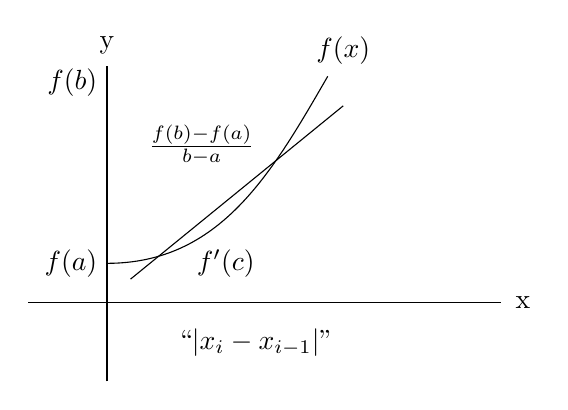
\begin{tikzpicture}
    		%ejes
    		\node[anchor=east] at (0.0,0.0) (origenreal) {}; %origen
    		\node at (-0.2,0.1) (origen) {};
  		%%%% EJES!!!
  		\draw [] (-1,0) -> (5,0);
  		\draw [] (0,-1) -> (0,3);
  		%%%PARABOLA
  		\node[anchor=east] at (0,0.5) (iii) {$f(a)$};
  		\node[anchor=east] at (3,3) (ddd) {};
  		\node[anchor=east] at (0, 2.8) (bbb) {$f(b)$};
		\node[anchor=east] at (2, 0.5) (fc) {$f'(c)$};
		\node[anchor=east] at (2,2) (fab) {$\frac{f(b)-f(a)}{b-a}$};
		\node[anchor=east] at (3, -0.5) () {``\(|x_i - x_{i-1}|\)''};
  		
  		\draw (iii) edge[-,out=0,in=240] (ddd);
  		%Recta
  		\draw [] (0.3,0.3) -> (3,2.5);
  		%\draw (invo) edge[->,out=90,in=270] (invy);
  		\node[anchor=east] at (5.5,0) (x) {x};
  		\node[anchor=north] at (0,3.5) (y) {y};
  		%funciones
  		\node at (3,3.2) (xy) {$f(x)$};
  		\node at (0.0, 2) (oy) {};
	\end{tikzpicture}
\end{center}

\vspace{0.5cm} %\newline \\
\raggedright
\underline{Def:} Sea \(\displaystyle e_i = |x_i - r|\) el error del paso \(i\) de un método iterativo. Si:

\begin{center}
	\begin{equation*}
		\lim_{i \to \infty} \frac{e_{i+1}}{e_i} = S < 1.
	\end{equation*}
\end{center} \\

Se dice que el método obedece `convergencia lineal'' con tasa \(S\).\\
\vspace{0.2cm}

\underline{Th:} Asuma que \(g(x)\) es continua y diferenciable, que \(g(r) = r\), y que \(S = |g'(r)| < 1\). Entonces la iteración de Punto Fijo converge linealmente con tasa \(S\) al punto fijo \(r\) para ``initial guesses" lo suficientemente cerca de $r$.\\
\vspace{0.2cm}
\underline{Dem:} Sea \(x_i\) el resultado de la iteración \(i\). De acuerdo al teorema del valor medio \(\left(f'(c) = \frac{(f(b) - f(a))}{(b-a)}\right)\)
\begin{center}
	\(g'(c_i) = \frac{(g(x_i) - g(r))}{x_i - r}\) \hspace{1cm} 
	\begin{equation*}
		\begin{aligned}
			a &= r \\ b &= x_i
		\end{aligned}
	\end{equation*}
	y recuerde \(x_{i+1} = g(x_i)\) y \(r = g(r)\)\\
	\vspace{0.2cm}
	$\Rightarrow g'(c_i) = \frac{(x_{i+1} - r)}{(x_{i} - r)}$\\
	\vspace{0.2cm}
	$\Rightarrow x_{i+1} - r = g'(c_i) \cdot (x_i - r)$\\
	\vspace{0.2cm}
	$\Rightarrow e_{i+1} = |g'(c_i)| \cdot e_i $\\
	\vspace{0.2cm}

	Si \(S = |g'(r)| \Rightarrow\) Existe un pequeño vecindario alrededor de r tal que para \(x \in [r - \epsilon, r + \epsilon] \Rightarrow |g'(x)| \leq \frac{S+1}{2}\) \\
	\vspace{1cm}
	$\Rightarrow$ \hspace{2cm} \(e_{i+1} = |g'(c_i)| \cdot e_i < \frac{S+1}{2} \cdot e_i\)\\
	\vspace{0.3cm}
	$\Rightarrow$ \hspace{1cm} \(\displaystyle\lim_{i \to \infty} \frac{e_{i+1}}{e_i} = \lim_{i \to 	\infty} |g'(c_i)| = |g'(r)| = S \) \hspace{0.5cm} $\square$ \\
	\vspace{1cm}
	$\Rightarrow e_{i+1} \approx S \cdot e_i$\\
	\vspace{1cm}
\end{center}
%Fin página 6

\raggedright

\underline{Def:} \hspace{0.1cm} Un método iterativo es llamado localmente convergente a ``\(r\)" si el método converge a \(r\) para ``initial guesses" suficientemente cercanos a \(r\).\\
\vspace{0.2cm}
En otras palabras, el metodo converge localmente a la raiz $r$, si existe la vecindad $(r - \epsilon, r + \epsilon )$, donde $\epsilon > 0$, de tal manera que que se de la convergencia a $r$ a partir detodas las estimaciones de la vecindad.
\vspace{0.2cm}

\subsection{Algunos teoremas utiles}
\underline{Th:} \textbf{Teorema de Taylor" (con residuo)}.\\
Sea ``\(x\)'' y ``\(x_0\)'' números reales, y ``\(f\)'' ``\(k+1\)'' - veces continua y diferenciable en el intervalo entre ``\(x\)'' y ``\(x_0\)'',
entonces existe un número ``\(c\)'' entre ``\(x\)'' y ``\(x_0\)'' tal que:\\
\begin{center}
	\begin{equation*}
	f(x) = f(x_0) + f'(x_0)\cdot(x-x_0) + \frac{f''(x_0)}{2!} \cdot (x-x_0)^2 + \cdots + 	\frac{f^{(k)}(x_0)}{k!} \cdot (x - x_0)^k + \frac{f^{(k+1)}(c)}{(k+1)!} \cdot (x - x_0)^{k+1}
	\end{equation*}
\end{center}
\vspace{0.5cm}

\underline{Th:} \textbf{Teorema del valor intermedio}.\\ 
\vspace{0.2cm}
Sea $f$ una funcion continua en un intervalo $ [a,b]$ , entonces $f$ reconoce cada valor entre $f(a)$ y $f(b)$. Es decir, si $y$ es un numero tal que  $f(a)< y < f(b)$, existe un numero $c$ de forma que $a < c < b \Rightarrow f(c) = y$   

\vspace{0.5cm}
\underline{Th:} \textbf{Teorema de Rolle}.\\

\vspace{0.2cm}
Sea $f$ una funcion continua y diferenciable en un intervalo $[a,b]$. Entonces existe un bumero $c$, entre $a$ y $b$ de tal forma que $\displaystyle f'(c) = \frac{f(a)- f(b)}{b-a}$

\vspace{0.5cm}
\underline{Th:} \textbf{Teorema de los limites continuos}.\\
\vspace{0.2cm}

Sea $f$ una funcion continua en las cercanias de $x_0$, y suponga que $\lim_{n \to \infty} x_n = x_0$. Entonces:\\
\begin{center}
	\begin{equation*}
		\lim_{n \to \infty} f(x_n) = f( lim_{n \to \infty} x_n ) = f(x_0) 
	\end{equation*}
\end{center}
En otras palabras los limites pueden trasladarse al interior de funciones continuas.

\newpage
\underline{Intro a Newton's Method} (o Newton - Raphson Method)\\
\begin{equation*}
	\begin{aligned}
		f(x) &= f(x_0) + f'(x_0) \cdot (x - x_0) + \frac{f''(c)}{2!} \cdot (x - x_0)^2  \\
		\\
		& \text{Considere si}\hspace{0.5cm} x = r, \text{la raíz.}\\
		\\
		f(r) &= f(x_0) + f'(x_0) \cdot (r-x_0) + \frac{f''(c)}{2!}\cdot (r-x_0)^2\\
		\\
		& x = r \Rightarrow f(r) = 0 \\
		\\
		0 &= f(x_0) + f'(x_0) \cdot (r - x_0) + \frac{f''(c)}{2!} \cdot (r - x_0)^2 \\
		\\
		& \text{¿Qué podemos hacer?}\\
		\\
		-f'(x_0)\cdot (r - x_0) &= f(x_0) + \frac{f''(c)}{2!} \cdot (r - x_0)^2 \\
		r - x_0 &= -(f'(x_0))^{-1} \cdot f(x_0) - (f'(x_0))^{-1} \cdot \frac{f''(c)}{2}\cdot (r - x_0)^2 \\
		\therefore r &= x_0 - (f'(x_0))^{-1}\cdot f(x_0) - (f'(x_0))^{-1}(f'(x_0))^{-1} \\
		\Rightarrow x_{i + 1} &= x_i - \frac{f(x_i)}{f'(x_i)} \\
		&= g_n(x_i)
	\end{aligned}
\end{equation*}

%Fin página 7
\newpage
\raggedright
\subsection{Metodo de Newton}

EL metodo de Newton, tambien conocido como Newton-Raphson. Por lo general converge mucho más rapido que lo dos metodos vistos anteriormente. Para encontrar una raiz $f(x) = 0 $, se da una estimacion inicial $x_0$ y se traza la recta tangente a la funcion $f$ en $x_0$. La recta tangente seguira en forma aproximada a la funcion hasta el eje $x$ hacia la raiz. El punto de inteseccion de la linea con el eje $x$ es una raiz aproximada, pero probablemente no es exacta si la $f$ es curva. Por lo tanto en este paso se itera.\\
\vspace{0.5cm}
\hspace{2.8cm}\textbf{Algoritmo:}\\ 	
\begin{center}
\(x_0\) = ``initial guess" \\
\hspace{1cm} \( \displaystyle x_{i+1} = x_i - \frac{f(x_i)}{f'(x_i)}\), \(i = 0, 1, ...\)
\end{center}
\vspace{0.5cm}
\begin{tabular}{c|c}
¿Recuerda? \(\begin{aligned}f(x) &= x^3 + x - 1\\ f'(x) &= 3x^2 + 1 \end{aligned}\) & \hspace{2cm}\begin{tabular}{l | c | c | r}
\(i\) & \(x_i\) & \(e_i\) & \(\frac{e_i}{e_{i-1}^2}\) \\
\hline
0 & -0.7  & 1.38  & -  \\
\hline
1 & 0.12  & 0.55  & 0.2906  \\
\hline
2 & 0.95  & 0.27  & 0.8933  \\
\hline
3 & 0.73  & 0.052  & 0.6924  \\
\hline
4 & 0.6845  & 0.0022  & 0.8214  \\
\hline
5 & 0.682332  & 0.00000437  & 0.8527  \\
\hline
6 & 0.68232780  & 0.00000000  &  0.8541 \\
\hline
7 & 0.68232780  & 0.00000000  &  ¿XXX? \\
\end{tabular}\\ \\
$\begin{aligned}\Rightarrow x_{i+1} &= x_i - \frac{x_{i}^3 + x - 1}{3x_{i}^2 + 1}\\ x_{i+1} &= \frac{2x_{i}^3 + 1}{3x_{i}^2 + 1}\end{aligned} $ & \\
\end{tabular}
\vspace{0.5cm}
\newline
\underline{Def:} Sea \(e_i\) el error de la iteración ``\(i\)". La iteración converge cuadráticamente si: \\
\begin{center}
\begin{equation*}
M = \lim_{i \to \infty} \frac{e_{i+1}}{e_{i}^2} < \infty 
\end{equation*}
\end{center}
\underline{Th:} Sea ``\(f\)" dos veces continuamente diferenciable y \(f(r) = 0\). Si \(f'(r) \neq 0\), entonces el método de Newton es local y cuadráticamente convergente a ``\(r\)". El error \(e_i\) en el paso \(i\) es: \\
\begin{center}
\begin{equation*}
\begin{split}
\lim_{i \to \infty} \frac{e_{i+1}}{e_{i}^2} = M\\
\text{donde}\\
M = \frac{|f''(r)|}{2|f'(r)|}
\end{split}
\end{equation*}
\end{center}
\vspace{1cm}
\underline{Demostración:} FPI con \(g(x) = x - \frac{f(x)}{f'(x)}\)
\begin{equation*}
\begin{split}
\Rightarrow g'(x) = 1 - \frac{f'(x)^2 - f(x) \cdot f''(x)}{f'(x)^2} = \frac{f(x) \cdot f''(x)}{f'(x)^2}\\
\text{pero} f(r) = 0  \hspace{0.5cm} \text{y} \hspace{0.5cm} f'(r) \neq 0 \\
\vspace{0.7cm}
\Rightarrow g'(r) = \frac{f(r) \cdot f''(r)}{(f'(r))^2} = 0
\end{split}
\end{equation*}
%Fin página 8
%\newpage
\raggedright
\subsection{Convergencia cuadrática:}
\begin{equation*}
\begin{aligned}
f(r) &= f(x_i) + f'(x_i) \cdot (r- x_i) + \frac{f''(c_i)}{2} \cdot (r - x_i)^2 \\
0 &= f(x_i) + (r - x_i) \cdot f'(x_i) + (r - x_i)^2 \cdot \frac{1}{2} \cdot f''(c_i) \\
\frac{-f(x_i)}{f'(x_i)} &= r - x_i + (r - x_i)^2 \cdot \frac{1}{2} \cdot \frac{f''(c_i)}{f'(x_i)}\\
x_i - r &= (r - x_i)^2 \cdot \frac{1}{2} \cdot \frac{f''(c_i)}{f'(x_i)} \\
\Rightarrow \frac{e_{i+1}}{e_{i}^2} &= \frac{1}{2} \cdot \frac{|f''(c_i)|}{|f'(x_i)|} \\
\therefore \lim_{i \to \infty} \frac{e_{i+1}}{e_{i}^2} &= \left| 2^{-1} \cdot \frac{f''(r)}{f'(r)}\right|
\end{aligned}
\end{equation*}
\underline{Def:} Asuma que \(r\) es una raíz de \(f\) y que \(f\) es diferenciable, esto es, asuma que \(f(r) = 0\). Entonces si \(0 = f(r) = f'(r) = \cdots = f^{(m-1)}(r)\), pero \(f^{(m)}(r) \neq 0\), decimos que \(f\) tiene una raíz de multiplicidad ``\(m\)'' en \(r\). Decimos que \(f\) tiene una raíz múltiple si \(m > 1\), en otro caso \((m = 1)\),  la raíz se dice que es simple.\\
%Fin página 4, faltan agregar las flechas
\subsection{Convergencia lineal del método de Newton:}
\vspace{0.8cm}
\raggedright\underline{Ex:} \hspace{0.5cm}\(f(x) = x^2\), \hspace{0.5cm}\(f(r) = 0 \hspace{0.5cm} \Rightarrow \hspace{0.5cm}  r = 0\) \\
\vspace{0.4cm}
$
\begin{aligned}
x_{i+1} &= x_i - \frac{f(x_i)}{f'(x_i)},\hspace{0.5cm} f'(x) = 2x \\
\hspace{0.4cm}\Rightarrow x_{i+1} &= x_i - \frac{x_{i}^2}{2 \cdot x_i}\\
&= \frac{x_i}{2}
\end{aligned}
$
\hspace{2cm}
\begin{tabular}{l | c | c | r}
\(i\) & \(x_i\) & \(e_i\) & \(\frac{e_i}{e_{i-1}}\) \\
\hline
0 & 1  & 1  & -  \\
\hline
1 & \(\frac{1}{2}\)  & 0.5  & 0.5  \\
\hline
2 & 0.25  & 0.25  & 0.5  \\
\hline
3 & 0.125  & 0.125  & 0.5  \\
\end{tabular}
\vspace{2cm}
\newline
\underline{Ex:} \hspace{1cm} \(f(x) = x^m\), \(f'(x) = m \cdot x^{m-1}\)\\
\vspace{0.5cm}
\hspace{1.5cm}\(\Rightarrow x_{i+1} = x_i - \frac{x_{i}^m}{m \cdot x_{i}^{m-1}} = \frac{m-1}{m} \cdot x_i\) \hspace{0.7cm}$\therefore$ Convergencia lineal... :'( \\
\vspace{0.5cm}
\underline{Th:} Asuma que \(f\) es una función \((m + 1)\) - veces continua y diferenciable en \([a,b]\) y tiene una multiplicidad ``\(m\)'' en la raíz ``\(r\)''. Entonces el método de Newton es localmente convergente a ``\(r\)'' y el error \(e_i\) es:\\
\begin{center}
\begin{equation*}
\lim_{i\to \infty} \frac{e_{i+1}}{e_i} = S = \frac{m-1}{m} \neq 0
\end{equation*}
\end{center}
\vspace{0.5cm}
%Fin página 9
\underline{Th:} Si \(f\) es \((m+1)\) - veces continua y diferenciable en \([a, b]\), donde hay una raíz ``\(r\)'' de multiplicidad \(m > 1\), entonces el método modificado de Newton\\
\begin{center}
\begin{equation*}
x_{i+1} = x_i - m \cdot \frac{f(x_i)}{f'(x_i)}
\end{equation*}
\end{center}
Converge local y cuadráticamente a ``\(r\)''.

\raggedright
\subsection{Método de la Secante:}
Como se vio en la seccion anterior el metodo de Newton converge mas rapido que el metodo de la biseccion y la iteracion de punto fijo. Esto se logra debido a que el metodo de Newton dispone de mas informacion(en particular, tiene la informacion entregada por la recta tangente de la funcion la cual se obtiene con la derivada).\\
Pero \textbf{¿que sucede si la derivada no esta disponible?}.\\
\vspace{0.2cm}
Para estos casos existe el metodo de la secante, el cual sustituye la recta tangente(derivada), por una aproximacion llamada recta secante!.\\

\vspace{0.8cm}
Reemplazando la derivada por nuestra aproximacion\\
\begin{equation*}
	f'(x) \approx \frac{f(x) - f(x - \Delta x)}{x - (x - \Delta x)} = \frac{f(x) - f(x-\Delta x)}{\Delta x}
\end{equation*}

Luego usando nuestra nueva aproximacion en el metodo de Newton\\
\begin{center}
	$ \textbf{\underline{metodo de Newton:}}\hspace{1cm} 
	\begin{aligned}
	x_0 &= \text{``initial guess''} \\
		x_{i+1} &= x_i - \frac{f(x_i)}{f'(x_i)}
	\end{aligned} 
	\vspace{0.5cm}
	\newline
	\vspace{0.5cm}
	\textbf{\underline{metodo de la secante:}}	
	\begin{aligned}
		x_0\hspace{0.1cm} \text{,} \hspace{0.1cm} x_1 &= \text{``initial guesses",} \hspace{0.5cm} x_0 \neq x_1 \\
	\hspace{1cm} x_{i+1} &= x_i - \frac{f(x_i) \cdot (x_i - x_{i-1})}{f(x_i) - f(x_{i-1})}
	\end{aligned}$
\end{center}
\hspace{2cm}
%fin pagina x
\newpage
Es posible demostrar que el metodo de la secante bajo el supuesto de que converge a $r$ y si \(f'(r) \neq 0 \), se cumple la relacion aproximada del error:\\
\begin{center}
$
\begin{aligned}
	 e_{i+1} &\approx \left|\frac{f''(r)}{2\cdot f'(r)}\right| \cdot e_i \cdot e_{i-1}\\	
	&= \left|\frac{f''(r)}{2 \cdot f'(r)}\right|^{\alpha -1} \cdot e_{i}^{\alpha}
\end{aligned}
$ \\
\end{center}
\vspace{0.5cm}
Donde, \(\alpha = \frac{1 + \sqrt{5}}{2} \approx 1.62\). La convergencia de este metodo se denomina convergencia super-lineal, lo cual significa que esta entre la convergencia de los metodos linealmente convergentes y los cuadraticamente convergentes.\\
\vspace{0.5cm}
\subsection{Criterios de parada}
\begin{enumerate}
 \Myitem $\displaystyle|x_{i+1} - x_i| < TOL$ \\
 \Myitem  $\displaystyle\frac{x_{i+1}- x_i}{x_{i+1}} < TOL$ \\  
 \Myitem $\displaystyle\frac{|x_{i+1} - x_i|}{\text{max}(|x_{i+1}|, \Theta)} < TOL$, por ejemplo $\Theta = 10^{-10}$
\end{enumerate}

%Fin página 10
%\newpage
\underline{Def:} Asuma que \(f\) es una función y que \(r\) es su raíz, i. e. \(f(r) = 0\). Asuma que \(x_a\) es una aproximación a \(r\).
Para el problema de encontrar una raíz, el backward-error de la aproximación \(x_a\) es \(|f(x_a) - 0|\) y el forward error es \(|x_a - r|\).\\
\vspace{0.2cm}
\begin{center}
\(f(r) = f(x_a) + f'(c) \cdot (r-x_a)\) \\
\vspace{0.3cm}
$\Rightarrow \underbrace{|(f(r) - f(x_a)|}_{\text{Backward - error}}$ = $|f'(c)| \cdot \underbrace{|r - x_a|}_{\text{Forward - error}}$ \\
\end{center}
\vspace{0.2cm}

Para esto nos damos como ejemplo una función $f(x) = x^3 - 2x^2 + \frac{4x}{3} - \frac{8}{27}$, donde podemos encontrar que una raiz de esta función es $r = \frac{2}{3}$, ya que  ($f(\frac{2}{3}) = (\frac{2}{3})^3 - 2\cdot (\frac{2}{3})^2 + \frac{4\cdot \frac{2}{3}}{3} - \frac{8}{27} = 0$). Si usamos algun metodo conocido para poder encontrar raices (por ejemplo, bisección), al encontrar valores aproximados cercanos a la raiz $x_a$ por cada iteración, y al evaluarla en la función ($f(x_a)$), podemos encontrar los backward y forward error correspondienes. Al realizar un grafico de backward y forward error a medida que hacemos iteraciones por bisección, encontramos lo siguiente:

\begin{python}
import numpy as np
import matplotlib.pyplot as plt

#funcion a utilizar para el ejemplo

def fun(x):
    return x**3 - 2*(x**2) + (4*x)/3 - (8./27)

#usaremos el metodo de la biseccion para ejemplo de FE y BE
def bisect(f, a, b, tol=10e-8):
    fa = f(a)
    fb = f(b)
    i = 0
    xa = []
    fxa = []
    
    if np.sign(f(a)*f(b)) >= 0:
        print('f(a)f(b)<0 not satisfied!')
        return None
    
    while(b-a)/2 > tol:
        c = (a+b)/2.
        fc = f(c)
        xa.append(c)
        fxa.append(fc)
        if fc == 0:
            break
        elif np.sign(fa*fc) < 0:
            b = c
            fb = fc
        else:
            a = c
            fa = fc
        i += 1
        
    xc = (a+b)/2.
    return xa,fxa

f = lambda x: x**3 - 2*(x**2) + (4*x)/3 - (8./27)
x = np.linspace(0.5,0.7,15)
y = []
xa = []
fxa = []
forward_error_grafico = []
backward_error_grafico = []
for i in range(0,len(x)):
    y.append(fun(x[i]))
xa,fxa = bisect(f, 0.5, 0.7)
iteration = []
for i in range(1,16):
    iteration.append(i)

for i in range(0,len(xa)):
    forward_error_grafico.append(abs((2/3.) - xa[i]))
for i in range(0,len(fxa)):
    backward_error_grafico.append(abs((f(2/3.)) - fxa[i]))

f, (ax1, ax2) = plt.subplots(1, 2, figsize=(15,5)) 
ax1.scatter(x, y)
ax1.plot(x,y,label='f (x)')
ax1.set_title('grafica f(x) con 15 puntos en intervalo [0.5 , 0.7]')
ax1.grid(True)
ax1.set_xlabel('eje x')
ax1.set_ylabel('eje y')
ax1.legend(loc=0)

ax2.set_xlabel('Iteration')
ax2.set_ylabel('Error')
ax2.semilogy(iteration, forward_error_grafico ,marker='o', linestyle='--', color='b',label='Forward error')
ax2.semilogy(iteration, backward_error_grafico ,marker='o', linestyle='--', color='r',label='Backward error')
ax2.grid(True)
ax2.set_title('Forward y Backward error con 15 iteraciones de f(x)')
ax2.legend(loc=0)

plt.savefig('images/fig1.pdf', format='pdf')
print(r"""
\begin{figure}[htbp]
    \centering
    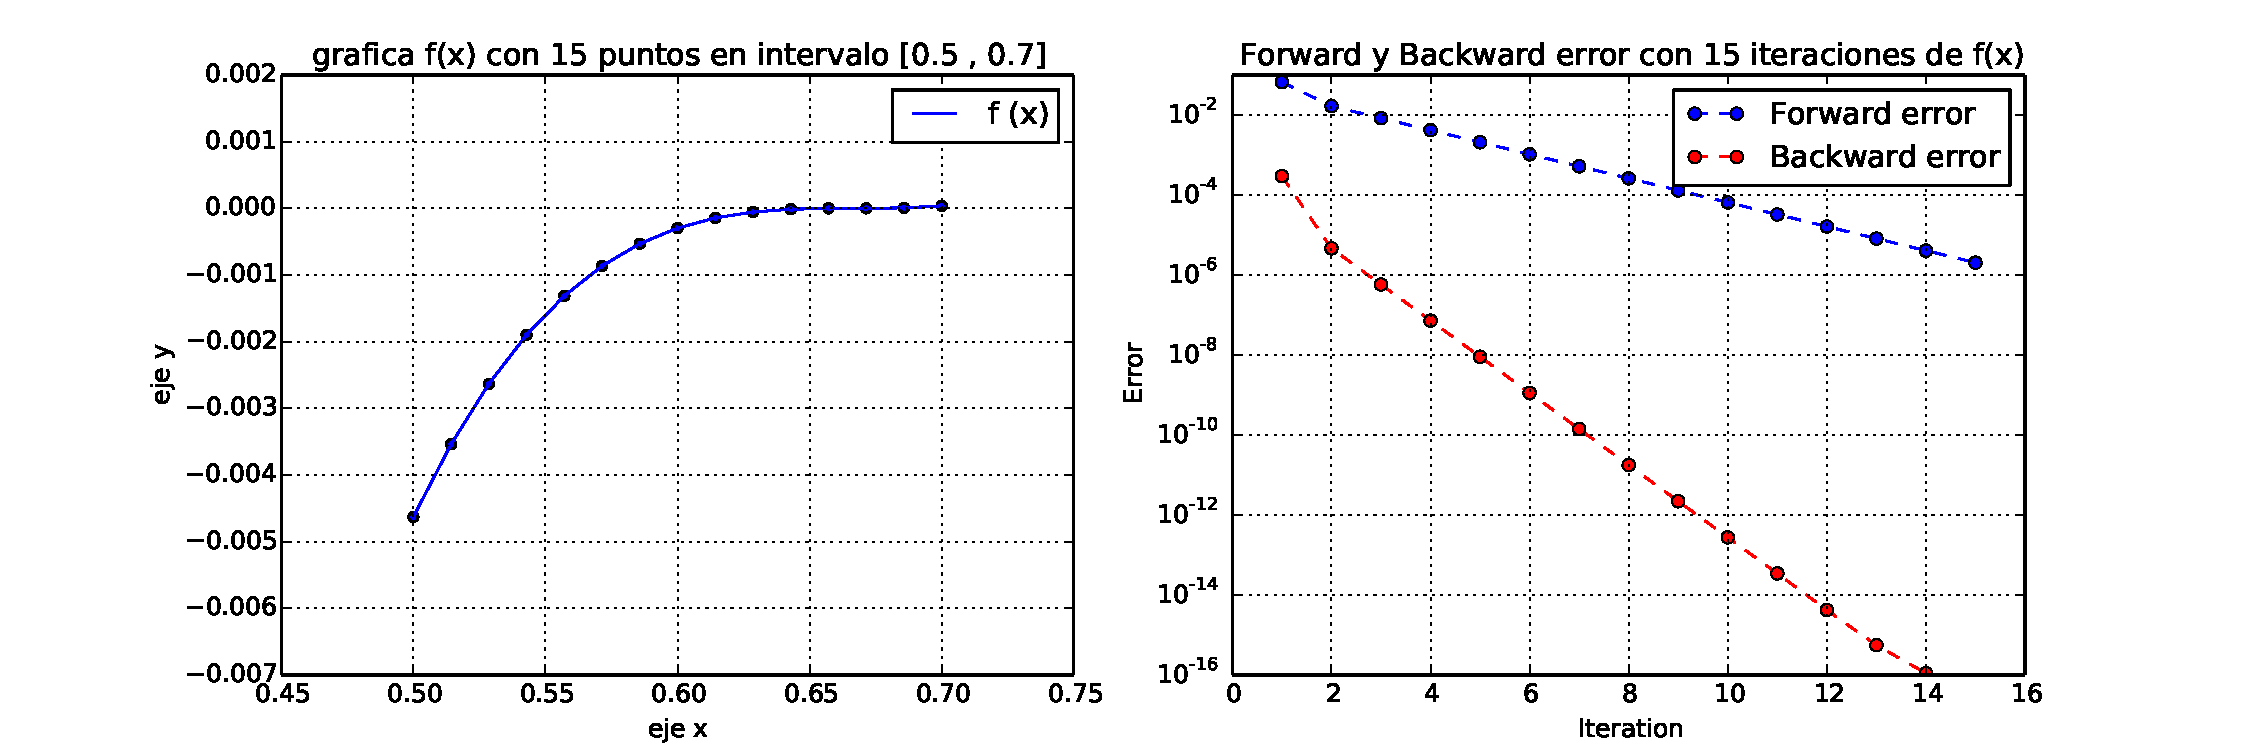
\includegraphics[width=18cm]{images/fig1.pdf}
    \label{fig:comparison}
\end{figure}
""")
\end{python}

Nos damos cuenta en el grafico que el backward error disminuye de forma mucho mas rapida que el forward error, es decir, si el backward error es pequeño, no implica que necesariamente el forward error es pequeño.
Lo que se quiere en búsqueda de ceros es que el forward error sea pequeño pero para poder medirlo necesitamos conocer la solución (¡que es precisamente lo que andamos buscando!) por lo cual lo que se hace es obtener al backward
error y concluir sobre el forward error. \\
\vspace{0.2cm}
Es \textbf{\color{red}¡¡¡MUY IMPORTANTE!!!} que se entienda este punto, \textbf{backward error pequeño no necesariamente implica forward error pequeño}, solo es válido cuando el problema es “bien condicionado”.

\vspace{0.2cm}
\begin{equation*}
\begin{aligned}
f(x_a) &= f(r) + f'(r) \cdot (r-x_a) + \cdots + \frac{f^{(m+1)}(c)}{(m+1)!} \cdot (r-x_a)^{m+1}\\
\Rightarrow & |f(r) - f(x_a)| = \left|\frac{f^{(m+1)}(c)}{(m+1)!}\right| \cdot |r-x_a|^m
\end{aligned}
\end{equation*}
%Fin página 11
%\newpage
\subsection{The Wilkinson polynomial (Wilkinson 1994)}
\begin{center}
\begin{equation*}
\begin{aligned}
W(x) &= \prod_{i = 1}^{20} (x-i) \text{, roots} = 1, 2, ..., 20\\
W(x) &= x^{20} - 210 \cdot x^{19} + \cdots + 1206647803780373360 \cdot x^6 + \cdots + 243 \cdots 000 (19 digitos) \\
\end{aligned}
\end{equation*}
\vspace{1cm}
$
\begin{aligned}
fzero(@wilkpoly, 16) \Rightarrow & 16.0148... \\ 
& 16.0000....0\\
&|x-x_a| \approx 10^{-2} 
\end{aligned}
$
\end{center}
\subsection{Sensitividad}
Problema: Encontrar \(r\), dado \(f(r) = 0\), para pequeñas perturbaciones agregadas \(\epsilon \cdot g(x), \epsilon << 1\)\\
\centering
$ \Rightarrow f(r + \Delta r) + \epsilon \cdot g(r + \Delta r) = 0 $ \\
\raggedright Expandiendo:\\
\begin{equation*}
\begin{aligned}
&f(r)+ \Delta r \cdot f'(r) + \epsilon \cdot g(r) + \epsilon \Delta r \cdot g'(r) + O(\Delta r^2) = 0 \\
\Rightarrow & \Delta r \approx \frac{-\epsilon \cdot g(r)}{f'(r) + \epsilon \cdot g'(r)} \hspace{0.3cm}\text{y asumiendo}\hspace{0.3cm} \epsilon g'(r) << f'(r) \\
& \Delta r \approx -\epsilon \cdot \frac{g(r)}{f'(r)}
\end{aligned}
\end{equation*}
%Fin página 12
\underline{Ex:}\hspace{1cm} Estime la sensitividad de \(r = 16\) para cambios en \(x^{15}\) \\
\vspace{0.5cm}
\text{donde:} 
\begin{equation*}
\begin{aligned}
W(x) &= \prod_{i = 1}^{20} (x -  i) = x^{20} + ... - 1672280820 \cdot x^{15} + \cdots \\
\Rightarrow W_{\epsilon}(x) &= W(x) + \epsilon \cdot g(x) ,\hspace{0.4cm} w'(16) = 15!4! \\
\Rightarrow \Delta r &= \frac{-\epsilon \cdot g(r)}{f'(r)} \approx \frac{16^{15} \cdot 1672280820}{15!4!} \cdot \epsilon \approx 6.14 \cdot 10^{13} \cdot \epsilon\\
\Rightarrow \Delta r & \approx 6.14 \cdot 10^{13} \cdot (\pm Emach) \\
&\approx 6.14 \cdot 10^{13} \cdot (\pm 2.22 \cdot 10^{-16}) \approx \pm 0.0136\\
&\approx |x-x_a|\\
\end{aligned}
\end{equation*}
%Fin página 13
\newpage
\subsection*{Condicionamiento (``primer encuentro")}
``Magnificación del error por parte del problema teórico"
\begin{equation*}
\begin{aligned}
K = \frac{\text{relative Forward error}}{\text{relative backward error}} = \frac{\frac{|x_a-r|}{|r|}}{\frac{|f(x_a) - f(r)|}{|f(r)|}} & \Rightarrow \frac{\frac{|\Delta r|}{|r|}}{|\frac{\Delta f}{f}|} = \frac{|f|}{|\frac{\Delta f}{\Delta r}|\cdot |r|} = \frac{\epsilon \cdot |g(r)|}{|r|\cdot |f'(r)|}\\
& \text{Donde}\hspace{0.3cm} f(r) + \epsilon \cdot g(r) = 0
\end{aligned}
\end{equation*}
\newline
\underline{Ex:} 
\begin{center}
\begin{equation*}
\begin{aligned}
x^2 - 2\cdot x + 1 &= 0 \hspace{0.5cm} \Leftrightarrow \hspace{0.5cm} (x-1)^2 = 0 \\
\Rightarrow x^2 - 2x + 1 - \epsilon &= 0 \\
\Rightarrow x_1 = 1 - \sqrt \epsilon \\
\Rightarrow x_2 = 1 + \sqrt \epsilon \\
\text{Si}\hspace{0.5cm} \epsilon \approx 10^{-8}\\
\Rightarrow x^2 - 2x + 1 - 10^{-8} &= 0 \\
x^2 - 2x + 0.99999999 &= 0 \\
\Rightarrow x_1 = 1 - 10^{-4} &= 0.9999 \\
x_2 = 1 + 10^{-4} &= 1.0001
\end{aligned}
\end{equation*}
\end{center}
\vspace{1cm}
Volviendo a \(W(x)\)
\begin{equation*}
K = \frac{|g(r)|}{|r||f'(r)|} = \frac{16^{15} \cdot 1672280820}{15! 4! 16} \approx 3.8 \cdot 10^{12}
\end{equation*}
\centering
$\Rightarrow$ Se espera perder ``12" dígitos de ``accuracy".\\
recuerda \(16 \approx 16.014...\)

\pagebreak
